% !TEX TS-program = pdflatex
% !TEX encoding = UTF-8 Unicode

% This is a simple template for a LaTeX document using the "article" class.
% See "book", "report", "letter" for other types of document.

\documentclass[11pt]{article} % use larger type; default would be 10pt

\usepackage[utf8]{inputenc} % set input encoding (not needed with XeLaTeX)

%%% Examples of Article customizations
% These packages are optional, depending whether you want the features they provide.
% See the LaTeX Companion or other references for full information.

%%% PAGE DIMENSIONS
\usepackage{geometry} % to change the page dimensions
\geometry{a4paper} % or letterpaper (US) or a5paper or....
% \geometry{margin=2in} % for example, change the margins to 2 inches all round
% \geometry{landscape} % set up the page for landscape
%   read geometry.pdf for detailed page layout information

\usepackage{graphicx} % support the \includegraphics command and options

% \usepackage[parfill]{parskip} % Activate to begin paragraphs with an empty line rather than an indent

%%% PACKAGES
\usepackage{booktabs} % for much better looking tables
\usepackage{array} % for better arrays (eg matrices) in maths
\usepackage{paralist} % very flexible & customisable lists (eg. enumerate/itemize, etc.)
\usepackage{verbatim} % adds environment for commenting out blocks of text & for better verbatim
%\usepackage{subfig} % make it possible to include more than one captioned figure/table in a single float
% These packages are all incorporated in the memoir class to one degree or another...

%%% HEADERS & FOOTERS
\usepackage{fancyhdr} % This should be set AFTER setting up the page geometry
\pagestyle{fancy} % options: empty , plain , fancy
\renewcommand{\headrulewidth}{0pt} % customise the layout...
\lhead{}\chead{}\rhead{}
\lfoot{}\cfoot{\thepage}\rfoot{}

%%% SECTION TITLE APPEARANCE
\usepackage{sectsty}
\allsectionsfont{\sffamily\mdseries\upshape} % (See the fntguide.pdf for font help)
% (This matches ConTeXt defaults)

%%% ToC (table of contents) APPEARANCE
\usepackage[nottoc,notlof,notlot]{tocbibind} % Put the bibliography in the ToC
\usepackage[titles,subfigure]{tocloft} % Alter the style of the Table of Contents
\renewcommand{\cftsecfont}{\rmfamily\mdseries\upshape}
\renewcommand{\cftsecpagefont}{\rmfamily\mdseries\upshape} % No bold!

\usepackage{amsmath}
\usepackage{listings}
\usepackage{xcolor}
\usepackage{subcaption}

\lstset{
    backgroundcolor=\color{red!10!green!10!blue!10},%代码块背景色为浅灰色
    rulesepcolor= \color{gray}, %代码块边框颜色
    breaklines=true,  %代码过长则换行
    numbers=left, %行号在左侧显示
    numberstyle= \small,%行号字体
    keywordstyle= \color{blue},%关键字颜色
    commentstyle=\color{gray}, %注释颜色
    frame=shadowbox%用方框框住代码块
}
%%% END Article customizations

%%% The "real" document content comes below...

\title{Implementation of Genetic Algorithm and Particle Swarm Optimization}
\author{Zhiyi Xia, Student ID:201794098}
%\date{} % Activate to display a given date or no date (if empty),
         % otherwise the current date is printed 

\begin{document}
\maketitle

\section{Impletmentation}


\subsection{Genetic Algorithm}
\begin{lstlisting}[language={Python}]
import numpy as np
import random
import time
import matplotlib.pyplot as plt
random.seed(time.time())
N = 4 * 3  # dna length
M = 15 # individual number
MAX_EPOCH = 100
Pc = 0.1
Pm = 0.01

def Main():
    indList = [genotype() for i in range(M)]
    initFit = [g.evaluate() for g in indList]
    fitRecord = []
    fitRecord.append(initFit)
    print('Initial Value:', initFit)

    for epoch in range(MAX_EPOCH):
        children = []
        random.shuffle(indList)
        for ind in indList:
            children.append(ind.mutation())
        for i in range(M//2):
            if flip(Pc):
                children += indList[i].cross1(indList[i + M//2])
            if flip(Pc):
                children += indList[i].cross2(indList[i + M//2])
        children += indList
	   # selection
        fitness = [-g.evaluate() for g in children]
        indList = random.choices(children, fitness, k=M)
        fitRecord.append([g.evaluate() for g in indList])

    # Result and Visualize
    [print(l) for l in fitRecord]
    plt.plot(list(range(MAX_EPOCH+1)), [np.max(x) for x in fitRecord])
    plt.show()

def target(x1, x2, x3):
    return 2 * x1 ** 2 - 3 * x2 ** 2 - 4 * x1 + 5 * x2 + x3

def flip(r):
    return random.random() < r

class genotype:
    def __init__(self):
        self. gene = []
        for i in range(N):
            self.gene.append(1 if flip(0.5) else 0)
        self.fitness = 0

    def evaluate(self):
        x1 = '0b' + ''.join(str(x) for x in self.gene[ :4])
        x2 = '0b' + ''.join(str(x) for x in self.gene[4:8])
        x3 = '0b' + ''.join(str(x) for x in self.gene[8:12])
        x1, x2, x3 = int(x1, 2), int(x2, 2), int(x3, 2)
        self.fitness = target(x1,x2,x3)
        return self.fitness

    def mutation(self):
        newInd = genotype()
        for i in range(len(self.gene)):
            if flip(Pm):
                newInd.gene[i] = (self.gene[i] + 1) % 2
            else:
                newInd.gene[i] = self.gene[i]
        return newInd

	# 1 point cross
    def cross1(self, pair):
        newInd1 = genotype()
        newInd2 = genotype()
        crossPoint = random.randint(1, len(self.gene) - 2)
        newInd1.gene[:crossPoint] = self.gene[:crossPoint].copy()
        newInd2.gene[:crossPoint] = pair.gene[:crossPoint].copy()
        newInd1.gene[crossPoint:] = pair.gene[crossPoint:].copy()
        newInd2.gene[crossPoint:] = self.gene[crossPoint:].copy()
        return newInd1, newInd2

	# 2 point cross
    def cross2(self, pair):
        newInd1 = genotype()
        newInd2 = genotype()
        P1 = random.randint(1, len(self.gene) - 2)
        P2 = random.randint(1, len(self.gene) - 2)
        if P1>P2:
            P1, P2 = P2, P1
        newInd1.gene[:P1] = self.gene[:P1].copy()
        newInd2.gene[:P1] = pair.gene[:P1].copy()
        newInd1.gene[P1:P2] = pair.gene[P1:P2].copy()
        newInd2.gene[P1:P2] = self.gene[P1:P2].copy()
        newInd1.gene[P2:] = self.gene[P2:].copy()
        newInd2.gene[P2:] = pair.gene[P2:].copy()
        return newInd1, newInd2
Main()
\end{lstlisting}

\subsection{Particle Swarm Optimitzation}
\begin{lstlisting}[language={Python}]
import numpy as np
import random
import time
import matplotlib.pyplot as plt
from mpl_toolkits.mplot3d import Axes3D
random.seed(time.time())

w = 0.8
c1 = 2
c2 = 2
N = 100
MAX_EPOCH = 30

def Main():
    particles = [Particle(random.random()*15, random.random()*15, random.random()*15) for x in range(N)]
    curve = []

    for epoch in range(MAX_EPOCH):
        if epoch % 5 == 0:
            x = [p.pos[0] for p in particles]
            y = [p.pos[1] for p in particles]
            z = [p.pos[2] for p in particles]
            plt.ion()
            fig = plt.figure(epoch+1)
            ax = fig.gca(projection='3d')
            plt.xlim(0,15)
            plt.ylim(0,15)
            ax.scatter(x,y,z)
            ax.set_zlim(0, 15)
            plt.show()

        particles[0].eval()
        maxFit = particles[0].fitness
        maxPos = particles[0].pos
        for p in particles[1:]:
            p.eval()
            if maxFit < p.fitness:
                maxFit = p.fitness
                maxPos = p.pos

        for p in particles:
            p.move(maxPos)
        curve.append(maxFit)
        print(maxPos,maxFit)
        print(np.mean([p.v for p in particles]))

    fig = plt.figure(0)
    plt.plot(curve)
    plt.pause(9999)




def eq(x1, x2, x3):
    return 2 * x1 ** 2 - 3 * x2 ** 2 - 4 * x1 + 5 * x2 + x3

def target(x1, x2, x3):
    t = eq(x1, x2, x3)
    return t

class Particle:
    def __init__(self, x1, x2, x3):
        self.pos = np.array([x1,x2,x3]).astype(np.float64)
        self.v = np.array([0,0,0]).astype(np.float64)
        self.fitness = target(*self.pos)
        self.posBest = np.array([x1,x2,x3])
        self.fitnessBest = target(*self.pos)

    def eval(self):
        self.fitness = target(*self.pos)
        if self.fitness>self.fitnessBest:
            self.fitnessBest = self.fitness
            self.posBest = self.pos.copy()
        return self.fitness

    def move(self, GlobalBest=None):
        self.v = w * self.v
        self.v += c1 * random.random() * (self.posBest - self.pos)
        self.v += c2 * random.random() * (GlobalBest - self.pos)

        self.pos += self.v
        self.pos[self.pos<0] = 0
        self.pos[self.pos>15] = 15
        self.eval()
        return self.fitness

Main()
\end{lstlisting}
\section{Experiment Result}
Our target is 
\begin{equation}
	\begin{aligned}
	&\mathop{\min}\ \ \ 2*x1^2 - 3*x2^2 - 4 *x1 + 5*x2 +x3 \\
	&\mathop{\max}\ \ \ 2*x1^2 - 3*x2^2 - 4 *x1 + 5*x2 +x3 \\
	&\text{s.t.}\ \  x1,x2,x3\ \in [0,15]
	\end{aligned}
\end{equation}
\subsection{Result of Genetic Algorithm}
Through mutiple times trying different combinations of parameters. My best result is 407 and -602. This program ran under mutation rate being 0.1, crossover rate being 0.01 and iteration being 1000.
\begin{figure*}[h]
\centering
\begin{minipage}[t]{0.48\textwidth}
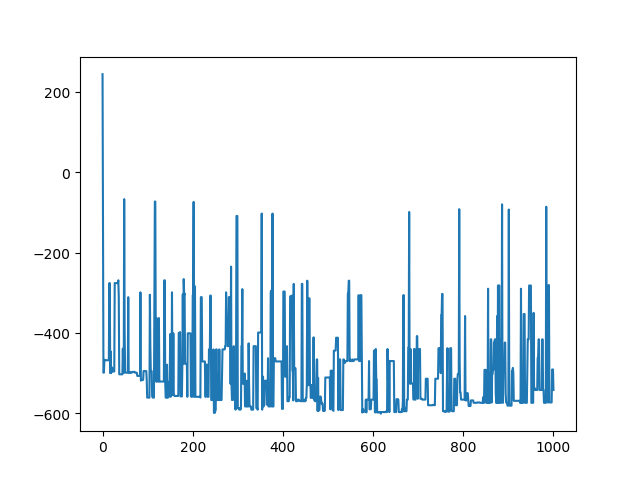
\includegraphics[scale=0.48]{GA_c0.1_m0.01_-602.png}
\caption{seeking minmuim using GA}
\end{minipage}
\begin{minipage}[t]{0.48\textwidth}
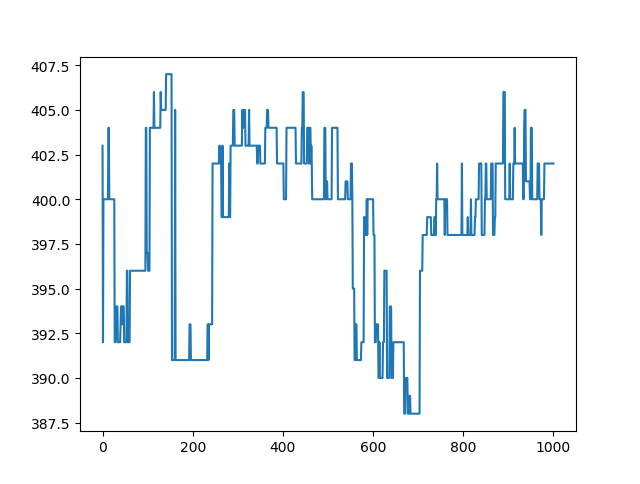
\includegraphics[scale=0.48]{GA_c0.1_m0.01_407.png}
\caption{seeking minmuim using GA}
\end{minipage}
\end{figure*}

\subsection{Result of PSO}
The max result of PSO is 407.08, here are the convergence curve and the particles' movement in first several epochs. The hyperparameters are $w = 0.5, c1=c2=2$.
\begin{figure*}[ht]
		\centering
	\subcaptionbox{Epoch 1}[0.3\linewidth]{
		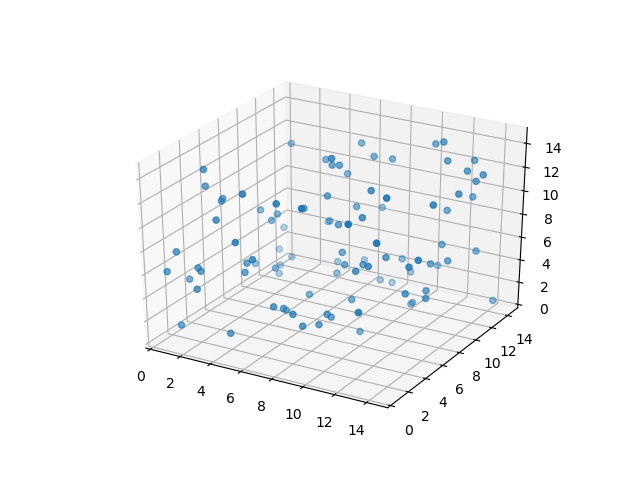
\includegraphics[scale=0.3]{PSO01.png}
	}
	\subcaptionbox{Epoch 2}[0.3\linewidth]{
		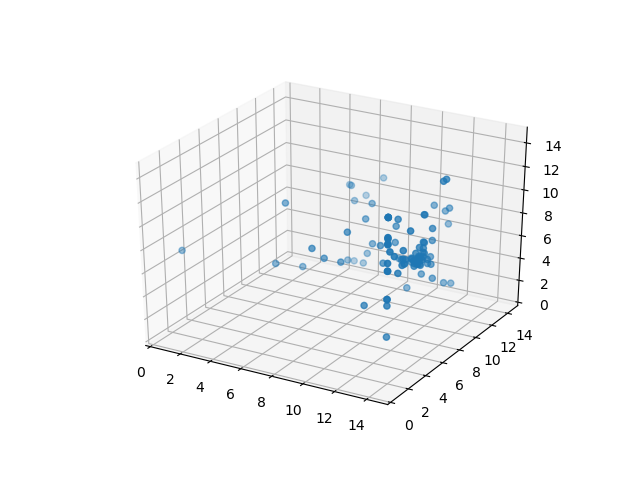
\includegraphics[scale=0.3]{PSO02.png}
	}
	\subcaptionbox{Epoch 3}[0.3\linewidth]{
		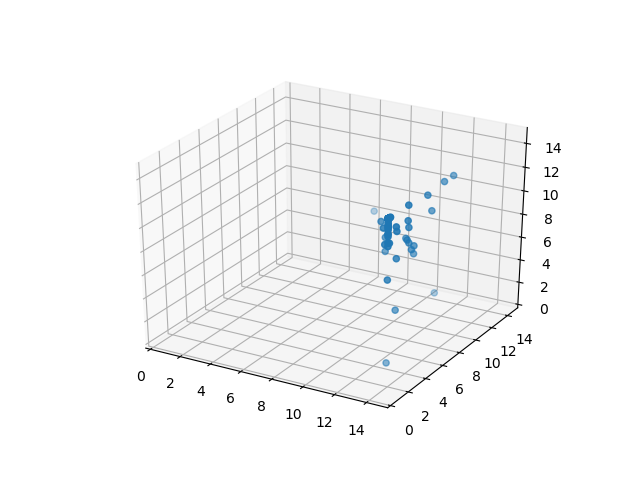
\includegraphics[scale=0.3]{PSO03.png}
	}
	\subcaptionbox{Epoch 4}[0.3\linewidth]{
		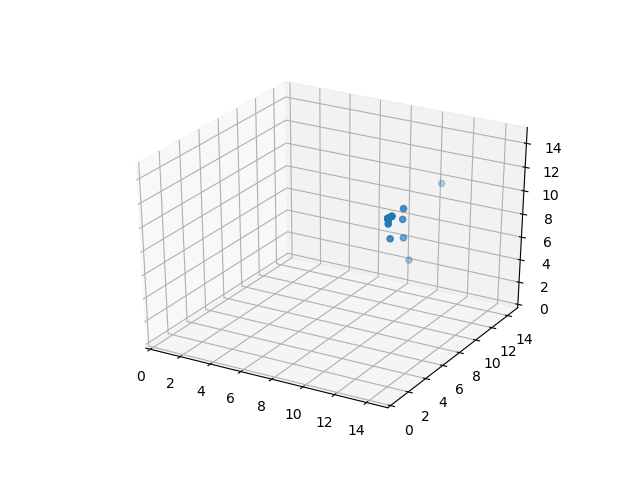
\includegraphics[scale=0.3]{PSO04.png}
	}
	\subcaptionbox{Epoch 5}[0.3\linewidth]{
		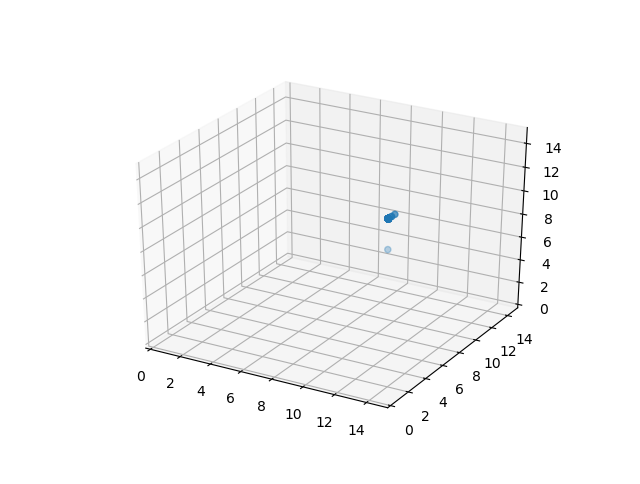
\includegraphics[scale=0.3]{PSO05.png}
	}
	\subcaptionbox{Convergence Curve}[0.3\linewidth]{
		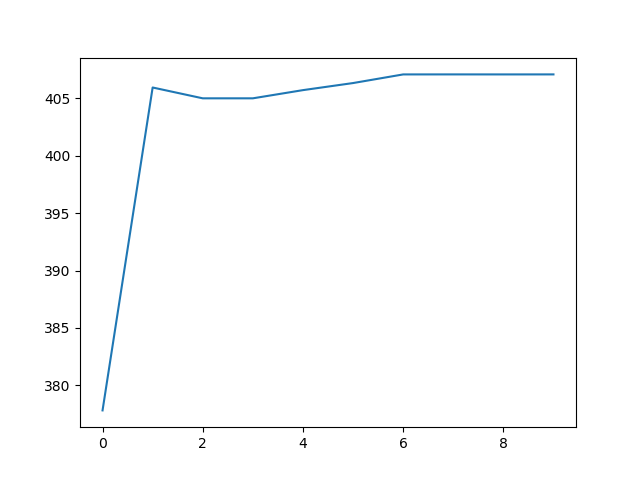
\includegraphics[scale=0.3]{PSO0.5_2_2.png}
	}
\end{figure*}

\section{Discussion}
\subsection{The adjustment of fitness value}
1. It has been experimented that raising the time of fitness will smooth the convergence curve and lowering the time of fitness will make the convergence curve more oscillating.
\begin{figure*}[htbp]
\centering
\begin{minipage}[t]{0.4\textwidth}
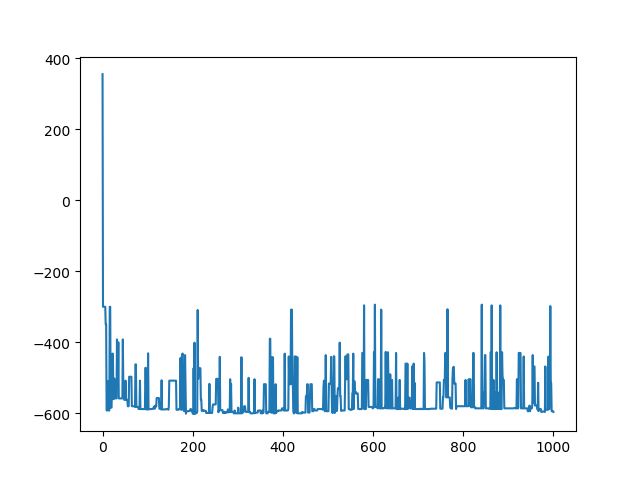
\includegraphics[scale=0.4]{3.png}
\caption{fitness times 3}
\end{minipage}
\begin{minipage}[t]{0.4\textwidth}
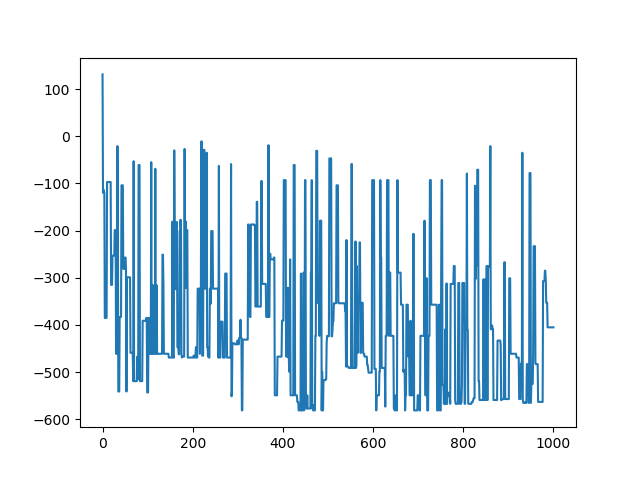
\includegraphics[scale=0.4]{1_3.png}
\caption{fitness times 1/3}
\end{minipage}
\end{figure*}
2. Additively nversing the fitness value will change maxmuim-seeking into minmuim-seeking
\subsection{About crossover}
If DNA pieces that 2 parents switched are excatly the same, then the crossover didn't make sense.
\subsection{About mutation}
1. If mutation rate is set to 0, then all the individuals will become the same and then the result will not change.
2. If mutation rate is set to 0.5, the convergence curve shake badly.
\begin{figure*}[htbp]
\centering
\begin{minipage}[t]{0.4\textwidth}
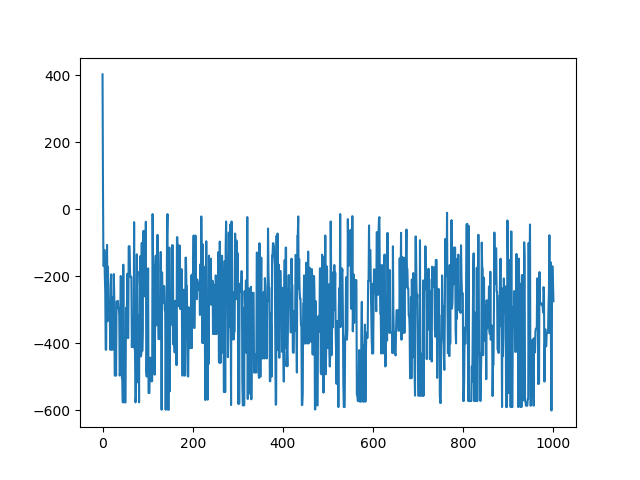
\includegraphics[scale=0.4]{m0.5.png}
\caption{mutation rate is 0.5}
\end{minipage}
\begin{minipage}[t]{0.4\textwidth}
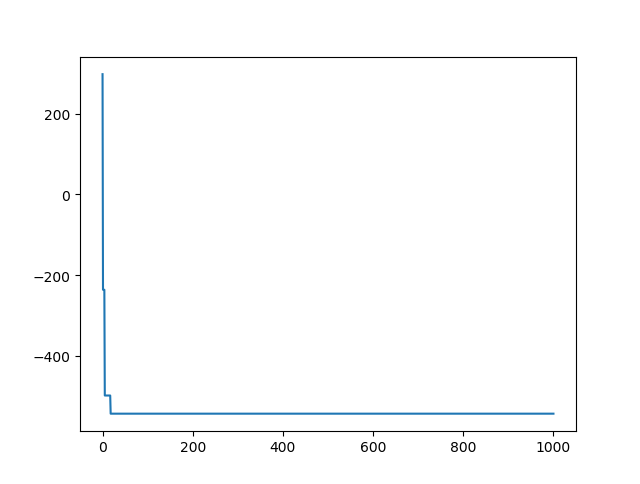
\includegraphics[scale=0.4]{0.png}
\caption{mutation rate is 0}
\end{minipage}
\end{figure*}


\end{document}
